\documentclass[10pt,a4paper]{article}
\usepackage[utf8]{inputenc}
\usepackage[T1]{fontenc}
\usepackage[numbers]{natbib}
\usepackage{color}
\usepackage{listings}
\usepackage{ amssymb }
\usepackage{courier}
\usepackage[pdftex]{graphicx}
\lstset{language=Haskell}
\lstset{breaklines=true}
\lstset{basicstyle=\scriptsize\sffamily}
\usepackage{url}
\usepackage{hyperref}


\newcommand{\sref}[1]{Section~\ref{#1}}
\newcommand{\annotate}[3]{
	\begin{scriptsize}
	\textcolor{#1}{\textbf{#2}~\textit{#3}}
	\end{scriptsize}\newline}
\newcommand{\todo}[1]{\annotate{red} {TODO:} {#1}}
\newcommand{\review}{\annotate{blue} {REVIEW:} {Please read the following, and make improvements. \newline}}

\author{
	Beerend Lauwers\\
	Utrecht University, The Netherlands}
\date{\today}
\title{Embedding Contract Inferencing for Functional Programs In Ask-Elle}
\begin{document}

\maketitle


\section{Abstract}
\todo{Finish up abstract}
Ask-Elle is a programming tutor created by Alex \citet{Gerdes:2012:phd} for his PhD Thesis. It utilizes (transformations of) model solutions to provide feedback to students on their progress.
However, if a student's program cannot be reduced to such a model solution, providing helpful feedback becomes hard to do. 
The Master Thesis of Jurri\"en \citet{Stutterheim:2013:thesis} focuses on the development of a contract inferencing system for functional programs, with the goal to embed this functionality in the Ask-Elle programming tutor, so as to provide a new source of meaningful feedback to students using the tutor.
In the "Future Work" section of the thesis, Stutterheim notes that the actual integration of the contract inferencing system in Ask-Elle still remains to be done.
This research proposal explores what needs to be done in order to attain that goal, as well as the effects it would have upon the tutor's capability to provide meaningful feedback.


5:58:09 PM] : ][CW][ : Brutos: whats your thesis about?
[5:58:14 PM] : ][CW][ : Brutos: well i guess about that :D
[5:58:18 PM] : ][CW][ : Brutos: but more in detail
[5:58:25 PM] =[BSID]= 1LT Beerdude26: Embedding contract inferencing in the Ask-Elle functional programming tutor
[5:58:39 PM] =[BSID]= 1LT Beerdude26: You know that everything has a type in Haskell
[5:58:50 PM] : ][CW][ : Brutos: yes
[5:59:26 PM] =[BSID]= 1LT Beerdude26: Contracts are a refinement of those (in fact, many researchers go the way of refinement types, but those need solvers and a whole lot of other crap)
[5:59:38 PM] =[BSID]= 1LT Beerdude26: So like, you have a function that goes from Int -> Int
[5:59:57 PM] =[BSID]= 1LT Beerdude26: You could define a contract for it that says "Input must be below 0, output must be below 2"
[6:00:10 PM] =[BSID]= 1LT Beerdude26: Or something like that, stupid example
[6:00:21 PM] =[BSID]= 1LT Beerdude26: You can use arbitrary functions when defining contracts
[6:00:30 PM] =[BSID]= 1LT Beerdude26: So it can also be that the input must be prime or something
[6:00:46 PM] =[BSID]= 1LT Beerdude26: Do you know about type inference?
[6:01:00 PM] : ][CW][ : Brutos: yes i did even learn one algorithm to do it
[6:01:04 PM] =[BSID]= 1LT Beerdude26: Algorithm W
[6:01:06 PM] =[BSID]= 1LT Beerdude26: Probably
[6:01:07 PM] : ][CW][ : Brutos: but i forgot everything about it again ._.
[6:01:07 PM] : ][CW][ : Brutos: :D
[6:01:49 PM] =[BSID]= 1LT Beerdude26: Well, the guy whose work I'm building on found out that for a subset of the Contract datatype he was using, it is possible to infer contracts for expressions, just like you can for types
[6:01:54 PM] : ][CW][ : Brutos: might be the notation in wiki looks somewhat familiar
[6:02:17 PM] : ][CW][ : Brutos: so i have some code and i can infer that id > 0
[6:02:18 PM] =[BSID]= 1LT Beerdude26: This is pretty nice; it allows you to define a "top-level" contract, and the rest of your code gets contracted appropriately
[6:02:36 PM] : ][CW][ : Brutos: oh i say my id > 0 and the compiler checks it everywhere?
[6:02:52 PM] =[BSID]= 1LT Beerdude26: Well
[6:03:41 PM] =[BSID]= 1LT Beerdude26: It's more like, "I know that this output comes from this function, and this output has the constraint that it must be at least 10 items long"
[6:04:01 PM] =[BSID]= 1LT Beerdude26: "So, I can infer that the constraint for the output of the function it came from must also be 10 items long"
[6:04:05 PM] =[BSID]= 1LT Beerdude26: Etc etc
[6:04:08 PM] =[BSID]= 1LT Beerdude26: Other tricks
[6:04:27 PM] =[BSID]= 1LT Beerdude26: In the end, you have very specific contracts for deeply nested code
[6:04:42 PM] : ][CW][ : Brutos: in 30 years it will make it into some kind of c++ standard :(
[6:04:50 PM] =[BSID]= 1LT Beerdude26: Which is nice, because that means you can find out more easily where your code is going wrong
[6:05:17 PM] =[BSID]= 1LT Beerdude26: The guy gave a nice example of insertion sort defined as a fold with insert: isort xs = foldr insert [] xs
[6:05:41 PM] =[BSID]= 1LT Beerdude26: Then he defined a contract: the input of xs doesn't matter as long as it's a list, the output of xs must be ordered.
[6:06:13 PM] =[BSID]= 1LT Beerdude26: Unfortunately, the inference does not support relations between input and output, so we can't say that the output must also be a permutation of the input
[6:06:33 PM] : ][CW][ : Brutos: is that a limitation of the theory or of the tools?
[6:06:38 PM] =[BSID]= 1LT Beerdude26: (Unless we transform our fold into paramorfism)
[6:06:58 PM] =[BSID]= 1LT Beerdude26: Of the theory, the inferencing algorithm is very simple
[6:07:15 PM] =[BSID]= 1LT Beerdude26: And cannot handle dependent functions
[6:07:24 PM] =[BSID]= 1LT Beerdude26: That's why people look to refinement types, because they do support all this
[6:07:37 PM] =[BSID]= 1LT Beerdude26: However, you need a constraint solver, some other fancy stuff
[6:07:44 PM] =[BSID]= 1LT Beerdude26: Proving it all is fucking hard
[6:07:52 PM] =[BSID]= 1LT Beerdude26: While proving this is pretty easy
[6:08:00 PM] =[BSID]= 1LT Beerdude26: At the moment, I'm doing code generation
[6:08:06 PM] : ][CW][ : Brutos: sounds like aweful big oh
[6:08:23 PM] =[BSID]= 1LT Beerdude26: Yeah it's probably pretty slow, too
[6:09:05 PM] =[BSID]= 1LT Beerdude26: The code generation I'm doing just takes Helium code (subset of Haskell 98 spec) and transforms it so it is fully contracted
[6:09:47 PM] =[BSID]= 1LT Beerdude26: At the moment, it's just generic contracts that always resolve to "true", so in other words the contracts don't impose any restraints whatsoever
[6:10:21 PM] =[BSID]= 1LT Beerdude26: However, I can then inject substitutions into the code generation bit
[6:10:37 PM] =[BSID]= 1LT Beerdude26: So then suddenly you have specific contracts that are being passed around
[6:11:34 PM] =[BSID]= 1LT Beerdude26: I think I'll copy this convo in my thesis text, it's a nice overview of what I have and have not done lol

\tableofcontents

\section{Introduction}
\todo{Talk about Ask-Elle and Juriens work}
In this thesis, we will extend the contract inferencing system developed by Jurri\"en Stutterheim and integrate it with the Ask-Elle programming tutor.

There are three main parts to this thesis:
firstly, the modifications to the original contract inferencing system are discussed and implemented. Secondly, code generation of contracted code is explained; Thirdly, the integration with the Ask-Elle programming tutor is laid out and developed.

\section{Problem description}
\subsection{Research question}
Having embedded contract inferencing in Ask-Elle, does this new functionality provide students with more detailed feedback than without?
Three main research goals are set up to achieve this.

\begin{description}
	\item{\textbf{Goal one}} Embed the contract inferencing system as described in Stutterheim's thesis.
	\item{\textbf{Goal two}} Perform tests with students to check if the newly-implemented functionality adds value to the provided feedback.
	\item{\textbf{Goal three}} Analyze the testing results and report our findings.
\end{description}

\subsubsection{Goal One: Embedding the contract inferencing system}

\begin{figure}[h]
  \centering
    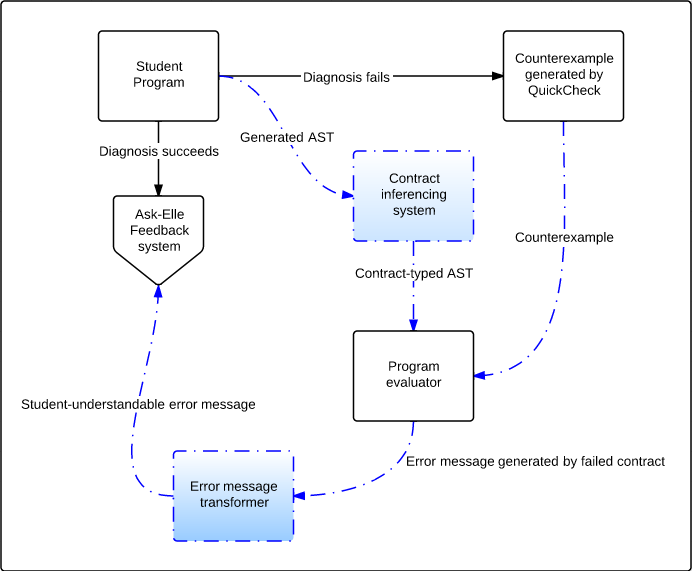
\includegraphics[width=0.5\textwidth]{Embed-Overview.png}
  \caption{Overview of steps involved in the contract inferencing system.}
\label{fig:EmbedOverview}
\end{figure}

Figure \ref{fig:EmbedOverview} depicts an overview of the steps involved in using the contract inferencing system.
The blue dashed-dotted arrows and boxes represent functionality that is not yet present in Ask-Elle, but is required for the contract inferencing system to be of use.
Let us step through the system and inspect the goals and requirements of each element in more detail.

Currently, if conventional 'diagnosis' of the student program fails, a QuickCheck example is generated, after which it is displayed to the user (this arrow is not shown).
Alongside the counterexample, the AST of the student program must be generated such that it can be used by the contract inferencing system.
The ASTs used by the Ask-Elle programming tutor and the contract inferencing system differ; Ask-Elle uses Helium as its back-end for Haskell, and Algorithm CW is based upon a small lambda language. So the first step towards embedding the system will be:

\begin{description}
	\item{\textbf{Step 1}} Modify and extend Algorithm CW to accept the AST generated by Ask-Elle, and embed it in Ask-Elle.
\end{description}

Initial work of this step has already been undertaken by research assistants (\todo{Who?}).
After completing Step 1, it should be possible to infer a contract for any arbitrary AST generated by Ask-Elle.

The next step is to use the contract-typed AST to generate an error message.
There are two ways of doing this:

\begin{enumerate}
	\item Use the QuickCheck-provided counterexample to transform the contract-typed AST directly, and then convert it back to an executable program and run it. We suspect that this functionality will be required for dependent function contracts.
	\item Convert the contract-typed AST back to an executable program immediately, and apply the counterexample to it.
\end{enumerate}

Replacing parts of the contract-typed AST with a counterexample was touched upon in Stutterheim's thesis, but an automated way of determining what should be replaced and where does not seem to be available.
Hence, this  is the next step:
\begin{description}
	\item{\textbf{Step 2}} Investigate an automated way of modifying the contract-typed AST with a counterexample, and implement this functionality.
\end{description}

After (not) modifying the contract-typed AST, it must be converted back into an executable program.
We assume the Helium-compiler has a way of feeding it an AST and returning an executable program.
However, keeping the well-known saying about assumptions in mind, we will have to investigate further:

\begin{description}
	\item{\textbf{Step 3}} Investigate if it is possible to feed a contract-typed AST to the Helium compiler. If not, investigate if this functionality can be implemented.
\end{description}

If all has gone well, we should end up with an error message generated by the Helium compiler, caused by a contract violation.
However, returning this error message to the student will not result in useful feedback.
Therefore, we must transform the error message by replacing the details of the contract violation with those of the function wrapped by the violated contract.
This transformed error message will be returned to the student. The final step of this subsection, then, is as follows:

\begin{description}
	\item{\textbf{Step 4}} Implement an error message transformer that "cleans up" the generated error message so it is understandable by the student, and feed it to the Ask-Elle feedback mechanism.
\end{description}

\subsubsection{Goal Two: Perform testing with students}

In August, Utrecht University hosts an Applied Functional Programming summer school.
This summer school course specifically targets students and participants who are not yet very knowledgeable about functional programming in general, and Haskell in particular.
This is an excellent opportunity to test the functionality described in Goal One.
Let us again go through each step that must be taken to complete this goal.

The first step is relatively simple, but nonetheless crucial:

\begin{description}
	\item{\textbf{Step 1}} Organize the practical aspects of the testing on time. Contact the coordinators of the summer school and request a time slot during which testing can take place.
\end{description}

After that, we must provide two versions of the Ask-Elle tutor: one with the new contract inferencing system embedded, and the original, unmodified one.
We require two versions to perform a simple A/B test: for each exercise, a version of Ask-Elle is randomly selected and presented to the student.
Thus, we require a way to randomly serve one of the versions to a student:

\begin{description}
	\item{\textbf{Step 2}} Prepare two versions of the Ask-Elle tutor, and set up access in such a way that, for each exercise, one of the versions is randomly served to the student.
\end{description}

After completing an exercise in Ask-Elle (there are around fifteen exercises in total), the student will fill out a very small survey if he or she encountered feedback containing a counterexample.
The feedback will be shown above the survey.
The following questions will then be visible below the feedback:

\fbox {
    \parbox{\linewidth}{
For each question, please mark the circle that corresponds with your opinion.
\begin{enumerate}
	\item The feedback above provided me with sufficient information to help me find the mistake in my code. \newline
[Strongly disagree] 0 - 0 - 0 - 0 - 0 [Strongly agree]
	\item The feedback above should indicate a more specific part of the code.\newline
[Strongly disagree] 0 - 0 - 0 - 0 - 0 [Strongly agree]
\end{enumerate}
    }
}

As this survey is quite small, it could be made multi-lingual if this makes students more inclined to take part in the survey.

With the results of these surveys, we are able to discern which version of Ask-Elle students prefer when they encounter feedback containing a counterexample.

So, our final steps for this goal are:

\begin{description}
	\item{\textbf{Step 3}} Build a small survey system that acquires any feedback containing a counterexample from the Ask-Elle tutor and presents the survey mentioned above, then writes the answers back to a database.
	\item{\textbf{Step 4}} Test the entire system beforehand, and ensure it is operational for use by the students.
	\item{\textbf{Step 5}} Collect survey results.
\end{description}

\subsubsection{Goal Three: Analyze the testing results and report findings}

Having collected the survey results, all that remains to be done is to analyze them and determine if the embedding of the contract inferencing system in Ask-Elle has increased the usefulness of feedback containing a counterexample provided to students, or not:

\begin{description}
	\item{\textbf{Step 1}} Analyze the survey results to answer the research question.
\end{description}

After processing the results, we will present our findings in a presentation, as is customary:

\begin{description}
	\item{\textbf{Step 2}} Report findings and problems encountered / lessons learned during this thesis in a presentation.
\end{description}

\section{Contract Inferencing}

\todo{Tell a bit about contract inferencing for functional languages}
\todo{Explain what problems there were with Jurriens code generation system and how you spent a month or two working it out}

\section{Providing richer feedback}

\todo{Explain modifications to typed-contracts}
\todo{Explain how we can't use QuickCheck properties that are predefined for many Ask-Elle exercises. It had to do with how QuickCheck properties may require dependent contracts if it takes more than a single input.}

\subsection{Using Ask-Elle's QuickCheck properties}


\section{Code Generation}

\review

Now that we have inferenced contracts for every function application, we can generate contracted code.

We go over the AST again and for every function definition X, we generate the following new functions:

\_\_contracted\_X
\_\_app\_X
\_\_final\_X

These functions ensure that all function calls are contracted. Let us go over what each one does.

\subsection{\_\_contracted\_X}
This function calls the assertPos function of the typed-contracts library, will dynamically assert the contract provided to it.


Let us look at the template:

\begin{lstlisting}
__contracted_X ctrt posinfo = assertPos [function info] (generatePositionData posinfo) ctrt funs
  where funs = [contracted function definition]
\end{lstlisting}

A generated function takes two arguments, ctrt and posinfo.
ctrt is a Contract that is passed to the assertPos function. 
Different function calls can thus have differing contracts assigned;
in other words, the generated function is polymorphic in its contract.

posinfo is simply a tuple of the line and column position of a function call, and is used to generate specific feedback at runtime if there is a contract violation.

There are two placeholders that are replaced during code generation:
the placeholder [function info] is replaced by a string that informs the user what kind of function violated its contract.
Two examples of such generated messages are:

"At the application of the higher-order function 'foldr'"
"At the application of the function 'insert'"

The other placeholder, [contracted function definition], is replaced by a contracted version of the original function.
For example, a contracted version of the identity function looks like this:

\begin{lstlisting}
fun (\__x01 -> __final_id __x01)
\end{lstlisting}

For each argument, an extra layer of fun is applied to capture them and make them available to the original function.

A higher-order argument requires a bit more work, as it self must be contracted before being passed to the original function.
For example,

\begin{lstlisting}
g f x = f x
\end{lstlisting}

will generate the following replacement for the [contracted function definition] placeholder:

\begin{lstlisting}
(fun (\ __x01 -> (fun (\ __x02 -> __final_g (\ a0 -> (appParam __x01 "first argument of parameter 1 of g" a0)) __x02))))
\end{lstlisting}

\todo{If we pass the string representation of the higher-order function to the \_\_contracted version, we can make this feedback richer.}

The \_\_contracted version of a function is referenced in the \_\_app version, which we will review next.

\subsection{\_\_app\_X}

This function captures information for use in feedback, wraps it appropriately, and passes it to the \_\_contracted version of the function.

Again, let us first examine the template:

\begin{lstlisting}
__app_X ctrt posinfo [argument patterns] = [applied arguments]
\end{lstlisting}

The arguments ctrt and posinfo appear here again: both are passed to the \_\_contracted version of the function. Note again that this generated function is polymorphic with respect to its contract.

The placeholders [argument patterns] and [applied arguments] are relatively simple.

[argument patterns] generates a triple for each argument, which contains a string representation of the argument, the position of the argument, and the argument itself.

[applied arguments] uses this extra information to provide richer feedback at runtime and applies the arguments to the contracted version of the function.

Let us revisit a previous example:

\begin{lstlisting}
g f x = f x
\end{lstlisting}

will generate the following code:
\begin{lstlisting}
__app_g ctrt posinfo (stra,posa,a) (strb,posb,b) =
 appParam (appParam (__contracted_g ctrt posinfo) (stra ++ generatePositionData posa) a) (strb ++ generatePositionData posb) b
\end{lstlisting}

The contracted version of the function is fed arguments using appParam, and are accompanied by feedback strings containing the argument as a string and its position in the source code.

\subsection{\_\_final\_X}

Lastly, this generated function ties everything together by transforming the original function definition, replacing normal function calls with their contracted equivalents.

For example, the foldr function is transformed into the following:

\begin{lstlisting}
__final_foldr f b (x:xs) = f x (__app_foldr [ctrt] [pos] (_,_,f) (_,_,b) (_,_,xs))
__final_foldr f b [] = b
\end{lstlisting}

We leave out the generated information for brevity.

Note how the recursive call is also contracted, and how f can consume its arguments in the normal manner while being a contracted function itself.

What about function applications that have higher-order arguments?

In those cases, the higher-order argument is not replaced with a call to its \_\_app version, but with a call to its \_\_contracted version.
For example, the expression

\begin{lstlisting}
foldr insert [] [5,4,7,0,10]
\end{lstlisting}

will generate the following \_\_final version:

\begin{lstlisting}
__app_foldr (_,_,__contracted_insert [ctrt] [pos]) (_,_,[]) (_,_,[5,4,7,0,10])
\end{lstlisting}

This expression is a good example of what the user will provide.
Of course, if the user provides a partially applied function, there is not much that can be done, in the same manner as the uncontracted version of the code.

\subsection{Other notes}
We have only given examples for named functions, but what about lambda functions? Our solution is quite simple: rename all lambda functions and place them in a where clause, after which code generation can proceed as normal.
Thus, anonymous functions are fully contracted as well, and can take part in contract inferencing and code generation.
\end{document}
